\documentclass[25pt, a0paper, landscape]{tikzposter}

% --- Font & Package Setup ---
\usepackage{fontspec}
\setmainfont{FreeSerif} 
\newfontfamily\bangla{FreeSerif}[Script=Bengali] % Add this specific line

\usepackage{amsmath}
\usepackage{graphicx}
\usepackage{booktabs}

% --- Color & Theme ---
\usetheme{Board} 
\colorlet{backgroundcolor}{white}

% --- Title Information ---
\title{The Scaled Dot-Product Attention Algorithm}
\author{Nazmul Hasan (ID: 2023100000130)}
\institute{Department of Computer Science, Southeast University}

\begin{document}

\maketitle

\begin{columns}
    % ================= COLUMN 1 =================
    \column{0.33}
    
    \block{Algorithm Overview}{
        The Scaled Dot-Product Attention algorithm is the foundation of modern sequence processing. This algorithm computes the contextual relationships between items in a sequence by processing the entire input simultaneously rather than sequentially. It works by taking a target element (the Query) and comparing it against a set of Key-Value pairs that represent the surrounding context. By calculating similarity scores, the algorithm assigns higher weights to the most relevant elements. This allows the system to easily capture long-range dependencies and understand the true meaning of a sequence, even if related words are far apart.
    }
    
    \block{Mathematical Formulation}{
        The Attention mechanism operates entirely through linear algebra and matrix multiplications. The foundational equation that dictates the algorithm's behavior is defined as:
        
        \vspace{0.4cm}
        $$\text{Attention}(Q, K, V) = \text{softmax}\left(\frac{QK^T}{\sqrt{d_k}}\right)V$$
        \vspace{0.4cm}
        
        \textbf{Variable Definitions:}
        \begin{itemize}
            \item $Q$ \textbf{(Query Matrix):} Mathematical representation of the current sequence item.
            \item $K$ \textbf{(Key Matrix):} Representations of all items serving as context.
            \item $V$ \textbf{(Value Matrix):} Matrices holding the actual semantic informational content.
            \item $d_k$ \textbf{(Dimension):} Vector length of the keys, used as a scaling denominator.
            \item $QK^T$\textbf{:} Dot product calculating raw similarity between Query and Keys. 
        \end{itemize}
    }

    \block{3. Step-by-Step Execution: Matrix Flow }{
        \textbf{Visual Simulation: "Bank River"} \\
        To see how the algorithm executes, we simulate a 2-word sequence. We want the algorithm to learn that "Bank" is related to water.
        
        \vspace{1cm}
        \textbf{Step 1: MatMul (Calculating Raw Scores)} \\
        The algorithm multiplies Query ($Q$) by transposed Key ($K^T$) to find the raw alignment score. Notice the high score (30) between Bank and River.
        $$Q \times K^T = \begin{bmatrix} q_{\text{bank}} \\ q_{\text{river}} \end{bmatrix} \times \begin{bmatrix} k_{\text{bank}} & k_{\text{river}} \end{bmatrix} = \begin{bmatrix} 10 & 30 \\ 5 & 20 \end{bmatrix}$$
        
        \vspace{1cm}
        \textbf{Step 2: Scale \& SoftMax (Converting to Weights)} \\
        Scores are divided by $\sqrt{d_k}$ and passed through Softmax to normalize rows into probabilities. Result: "Bank" pays \textbf{90\% of its attention} to "River".
        $$\text{Softmax}\left( \frac{\text{Scores}}{\sqrt{d_k}} \right) = \begin{bmatrix} 0.10 & \mathbf{0.90} \\ 0.20 & 0.80 \end{bmatrix}$$

        {
        \textbf{Step 3: MatMul with V (Final Context)} \\
        Probability weights are multiplied by the Value ($V$) matrix. The embedding for "Bank" is now heavily infused with the meaning of "River".
        $$\begin{bmatrix} 0.10 & 0.90 \\ 0.20 & 0.80 \end{bmatrix} \times \begin{bmatrix} v_{\text{bank}} \\ v_{\text{river}} \end{bmatrix} = \begin{bmatrix} 0.10(v_{\text{bank}}) + \mathbf{0.90(v_{\text{river}})} \\ 0.20(v_{\text{bank}}) + 0.80(v_{\text{river}}) \end{bmatrix}$$
    }
    }

    % ================= COLUMN 2 =================
    \column{0.33}
    
    {
    
    }

    \block{4. Diagrams \& Visualizations}{
        \begin{center}
            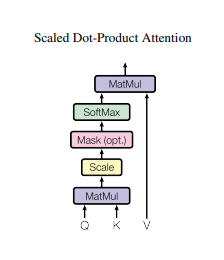
\includegraphics[width=0.6\linewidth]{scaled dot product attention.png}
            \vspace{0.5cm}\\
            \textit{Fig 1: Scaled Dot-Product Attention architecture (Vaswani et al., 2017).}
        \end{center}
    }

    \block{5. Time \& Space Complexity}{
        \textit{Let \textbf{$N$} = Sequence Length and \textbf{$d$} = Embedding Dimension.}

        \vspace{0.4cm}
        \textbf{1. Time Complexity Breakdown: $\mathcal{O}(N^2 \cdot d)$}
        \begin{itemize}
            \item \textbf{Phase A: Alignment Scores ($Q \times K^T$)} \\
            \textit{Shapes:} $[N \times d] \times [d \times N] \rightarrow \mathbf{[N \times N]}$. Requires $d$ multiplications across $N^2$ elements. Cost: $\mathcal{O}(N^2 \cdot d)$
            
            \item \textbf{Phase B: Scaling and Softmax} \\
            Scales and normalizes the resulting grid. Cost: $\mathcal{O}(N^2)$
            
            \item \textbf{Phase C: Contextual Output (Weights $\times V$)} \\
            \textit{Shapes:} $[N \times N] \times [N \times d] \rightarrow \mathbf{[N \times d]}$. Cost: $\mathcal{O}(N^2 \cdot d)$
        \end{itemize}
        
        \vspace{0.2cm}
        \textbf{Conclusion:} Quadratic scaling ($N^2$) is why processing extremely long documents requires massive computational power.

        \vspace{0.6cm}

        \textbf{2. Space (Memory) Complexity: $\mathcal{O}(N^2 + N \cdot d)$}
        \begin{itemize}
            \item \textbf{Storing the Inputs:} Holding $Q$, $K$, and $V$ matrices costs $\mathcal{O}(N \cdot d)$.
            \item \textbf{The Bottleneck:} The algorithm must instantly instantiate and store the entire $N \times N$ raw alignment grid in memory before it can apply Softmax. Cost: $\mathcal{O}(N^2)$.
        \end{itemize}
    }

    \block{6. Real-World Application: Machine Translation}{
        \textbf{Resolving Polysemy in NMT Systems} \\
        When translating \textit{"I sat on the bank of the river"} into Bengali, sequential models often confuse "bank" as financial ({\bangla ব্যাংক}) vs. river side ({\bangla নদীর তীর}). SDPA resolves this contextually:

        }

    % ================= COLUMN 3 =================
    \column{0.34}
    \block{6. Real-World Application (Continued)}{
    \normalsize \color{black} % Medium size and Black color
    \vspace{0.4cm}
    \textbf{Step-by-Step Execution:}
    
    \begin{enumerate}
        \item Querying: Sets the ambiguous word "bank" as the active Query ($Q$).
        \item Contextual Scanning: Compares $Q$ against all words (Keys). Math finds the highest alignment match between "bank" and "river."
        \item Semantic Fusion: Updates the vector for "bank" to include the data for "river."
        \item Output: The system confidently translates to: ({\bangla নদীর তীর}).
    \end{enumerate}
}

    \block{7. Case Study \& Matrix Simulation}{
        \textbf{Coreference Resolution (The Pronoun Problem)} \\
        \textit{"The animal didn't cross the street because \textbf{it} was too tired."} \\
        How does the computer know \textbf{"it"} refers to the animal?
        
        \vspace{0.3cm}
        \textbf{Step A: The Dot Product ($Q \times K^T$)} \\
        The Query for "it" ($q_{\text{it}}$) finds strong alignment with "animal" ($k_{\text{animal}}$) because the context contains "tired".
        \[
        q_{\text{it}} \times \begin{bmatrix} k_{\text{animal}} & k_{\text{street}} & k_{\text{it}} \end{bmatrix} = \begin{bmatrix} \mathbf{5.0} & 1.0 & 2.0 \end{bmatrix}
        \]
        
        \vspace{0.3cm}
        \textbf{Step B: Softmax Normalization} \\
        The dominant score ($e^{5.0}$) results in \textbf{93\% attention} assigned to "animal".
        \[
        \text{Softmax}\left(\dots\right) = \begin{bmatrix} \mathbf{0.93} & 0.02 & 0.05 \end{bmatrix}
        \]
        
        \vspace{0.3cm}
        \textbf{Step C: Semantic Fusion} \\
        Weights are multiplied by Value vectors ($V$). Result: "it" is now \textbf{93\% animal}.
        \[
        \begin{bmatrix} \mathbf{0.93} & 0.02 & 0.05 \end{bmatrix} \times \begin{bmatrix} v_{\text{animal}} \\ v_{\text{street}} \\ v_{\text{it}} \end{bmatrix} = \mathbf{0.93(v_{\text{animal}})} + \dots
        \]
    }

         \block{8. Algorithm Comparison}{
        \normalsize \color{black} % Medium-level font and black color
        \vspace{0.5cm}
        \begin{center}
        \resizebox{\linewidth}{!}{
        \renewcommand{\arraystretch}{1.8} % Increased spacing to make the table feel "bigger"
        \begin{tabular}{l l l l l}
        \toprule
        \textbf{Feature} & \textbf{CNN} & \textbf{RNN} & \textbf{LSTM} & \textbf{Self-Attention (Transformer)} \\
        \midrule
        Primary Use & Image processing & Sequential data & Long-term dependencies & NLP, vision tasks \\
        Processing Style & Spatial hierarchies & Sequential & Sequential with memory & Parallelized \\
        Long-Term Context & No & Limited & Yes & Yes (Simultaneous) \\
        Training Speed & Fast & Slow & Slower & Fast (parallel matrix math) \\
        Scalability & High & Low & Moderate & Very high \\
        \bottomrule
        \end{tabular}
        }
        \end{center}
    }

    \block{References}{
        \large \color{black} % Large font size for easy visibility and black color
        \begin{itemize}
            \item [1] Vaswani, A., et al. (2017). Attention is all you need. \textit{NIPS}, 30.
            \item [2] Devlin, J., et al. (2018). BERT. \textit{arXiv:1810.04805}.
            \item [3] Smith, E. "CNN vs RNN vs LSTM vs Transformer". \textit{Medium}.
        \end{itemize}
    }
\end{columns}

\end{document}